\documentclass[]{article}
\usepackage{lmodern}
\usepackage{amssymb,amsmath}
\usepackage{ifxetex,ifluatex}
\usepackage{fixltx2e} % provides \textsubscript
\ifnum 0\ifxetex 1\fi\ifluatex 1\fi=0 % if pdftex
  \usepackage[T1]{fontenc}
  \usepackage[utf8]{inputenc}
\else % if luatex or xelatex
  \ifxetex
    \usepackage{mathspec}
  \else
    \usepackage{fontspec}
  \fi
  \defaultfontfeatures{Ligatures=TeX,Scale=MatchLowercase}
\fi
% use upquote if available, for straight quotes in verbatim environments
\IfFileExists{upquote.sty}{\usepackage{upquote}}{}
% use microtype if available
\IfFileExists{microtype.sty}{%
\usepackage{microtype}
\UseMicrotypeSet[protrusion]{basicmath} % disable protrusion for tt fonts
}{}
\usepackage[margin=1in]{geometry}
\usepackage{hyperref}
\hypersetup{unicode=true,
            pdftitle={Crashkurs Datenanalyse mit R},
            pdfauthor={Sebastian Sauer},
            pdfborder={0 0 0},
            breaklinks=true}
\urlstyle{same}  % don't use monospace font for urls
\usepackage{color}
\usepackage{fancyvrb}
\newcommand{\VerbBar}{|}
\newcommand{\VERB}{\Verb[commandchars=\\\{\}]}
\DefineVerbatimEnvironment{Highlighting}{Verbatim}{commandchars=\\\{\}}
% Add ',fontsize=\small' for more characters per line
\usepackage{framed}
\definecolor{shadecolor}{RGB}{248,248,248}
\newenvironment{Shaded}{\begin{snugshade}}{\end{snugshade}}
\newcommand{\AlertTok}[1]{\textcolor[rgb]{0.94,0.16,0.16}{#1}}
\newcommand{\AnnotationTok}[1]{\textcolor[rgb]{0.56,0.35,0.01}{\textbf{\textit{#1}}}}
\newcommand{\AttributeTok}[1]{\textcolor[rgb]{0.77,0.63,0.00}{#1}}
\newcommand{\BaseNTok}[1]{\textcolor[rgb]{0.00,0.00,0.81}{#1}}
\newcommand{\BuiltInTok}[1]{#1}
\newcommand{\CharTok}[1]{\textcolor[rgb]{0.31,0.60,0.02}{#1}}
\newcommand{\CommentTok}[1]{\textcolor[rgb]{0.56,0.35,0.01}{\textit{#1}}}
\newcommand{\CommentVarTok}[1]{\textcolor[rgb]{0.56,0.35,0.01}{\textbf{\textit{#1}}}}
\newcommand{\ConstantTok}[1]{\textcolor[rgb]{0.00,0.00,0.00}{#1}}
\newcommand{\ControlFlowTok}[1]{\textcolor[rgb]{0.13,0.29,0.53}{\textbf{#1}}}
\newcommand{\DataTypeTok}[1]{\textcolor[rgb]{0.13,0.29,0.53}{#1}}
\newcommand{\DecValTok}[1]{\textcolor[rgb]{0.00,0.00,0.81}{#1}}
\newcommand{\DocumentationTok}[1]{\textcolor[rgb]{0.56,0.35,0.01}{\textbf{\textit{#1}}}}
\newcommand{\ErrorTok}[1]{\textcolor[rgb]{0.64,0.00,0.00}{\textbf{#1}}}
\newcommand{\ExtensionTok}[1]{#1}
\newcommand{\FloatTok}[1]{\textcolor[rgb]{0.00,0.00,0.81}{#1}}
\newcommand{\FunctionTok}[1]{\textcolor[rgb]{0.00,0.00,0.00}{#1}}
\newcommand{\ImportTok}[1]{#1}
\newcommand{\InformationTok}[1]{\textcolor[rgb]{0.56,0.35,0.01}{\textbf{\textit{#1}}}}
\newcommand{\KeywordTok}[1]{\textcolor[rgb]{0.13,0.29,0.53}{\textbf{#1}}}
\newcommand{\NormalTok}[1]{#1}
\newcommand{\OperatorTok}[1]{\textcolor[rgb]{0.81,0.36,0.00}{\textbf{#1}}}
\newcommand{\OtherTok}[1]{\textcolor[rgb]{0.56,0.35,0.01}{#1}}
\newcommand{\PreprocessorTok}[1]{\textcolor[rgb]{0.56,0.35,0.01}{\textit{#1}}}
\newcommand{\RegionMarkerTok}[1]{#1}
\newcommand{\SpecialCharTok}[1]{\textcolor[rgb]{0.00,0.00,0.00}{#1}}
\newcommand{\SpecialStringTok}[1]{\textcolor[rgb]{0.31,0.60,0.02}{#1}}
\newcommand{\StringTok}[1]{\textcolor[rgb]{0.31,0.60,0.02}{#1}}
\newcommand{\VariableTok}[1]{\textcolor[rgb]{0.00,0.00,0.00}{#1}}
\newcommand{\VerbatimStringTok}[1]{\textcolor[rgb]{0.31,0.60,0.02}{#1}}
\newcommand{\WarningTok}[1]{\textcolor[rgb]{0.56,0.35,0.01}{\textbf{\textit{#1}}}}
\usepackage{graphicx,grffile}
\makeatletter
\def\maxwidth{\ifdim\Gin@nat@width>\linewidth\linewidth\else\Gin@nat@width\fi}
\def\maxheight{\ifdim\Gin@nat@height>\textheight\textheight\else\Gin@nat@height\fi}
\makeatother
% Scale images if necessary, so that they will not overflow the page
% margins by default, and it is still possible to overwrite the defaults
% using explicit options in \includegraphics[width, height, ...]{}
\setkeys{Gin}{width=\maxwidth,height=\maxheight,keepaspectratio}
\usepackage[normalem]{ulem}
% avoid problems with \sout in headers with hyperref:
\pdfstringdefDisableCommands{\renewcommand{\sout}{}}
\IfFileExists{parskip.sty}{%
\usepackage{parskip}
}{% else
\setlength{\parindent}{0pt}
\setlength{\parskip}{6pt plus 2pt minus 1pt}
}
\setlength{\emergencystretch}{3em}  % prevent overfull lines
\providecommand{\tightlist}{%
  \setlength{\itemsep}{0pt}\setlength{\parskip}{0pt}}
\setcounter{secnumdepth}{0}
% Redefines (sub)paragraphs to behave more like sections
\ifx\paragraph\undefined\else
\let\oldparagraph\paragraph
\renewcommand{\paragraph}[1]{\oldparagraph{#1}\mbox{}}
\fi
\ifx\subparagraph\undefined\else
\let\oldsubparagraph\subparagraph
\renewcommand{\subparagraph}[1]{\oldsubparagraph{#1}\mbox{}}
\fi

%%% Use protect on footnotes to avoid problems with footnotes in titles
\let\rmarkdownfootnote\footnote%
\def\footnote{\protect\rmarkdownfootnote}

%%% Change title format to be more compact
\usepackage{titling}

% Create subtitle command for use in maketitle
\newcommand{\subtitle}[1]{
  \posttitle{
    \begin{center}\large#1\end{center}
    }
}

\setlength{\droptitle}{-2em}
  \title{Crashkurs Datenanalyse mit R}
  \pretitle{\vspace{\droptitle}\centering\huge}
  \posttitle{\par}
  \author{Sebastian Sauer}
  \preauthor{\centering\large\emph}
  \postauthor{\par}
  \predate{\centering\large\emph}
  \postdate{\par}
  \date{2017-05-16}


\begin{document}
\maketitle

Nicht jeder liebt Datenanalyse und Statistik\ldots{} in gleichem Maße.
Das ist zumindest meine Erfahrung aus dem Unterricht :neckbeard: :fire:.
Crashkurse zu R sind vergleichbar zu Crahskursen zu Französisch - kann
man machen, aber es sollte die Maxime gelten ``If everything else
fails''.

Dieser Crashkurs ist für Studierende oder Anfänger der Datenanalyse
gedacht, die in kurzer Zeit einen verzweifelten Versuch \ldots{} äh
\ldots{} einen grundständigen Überblick über die Datenanalyse erwerben
wollen.

Ok, also los geht's im Schweingalopp durch die Datenanalyse :notes:
:dancer:.

\hypertarget{software}{%
\section{Software}\label{software}}

Bevor wir uns die Schritte näher anschauen, ein paar Worte zur Software.

\hypertarget{programme}{%
\subsection{Programme}\label{programme}}

Wir brauchen zwei Programme.

\begin{itemize}
\tightlist
\item
  R
\item
  RStudio
\end{itemize}

Wenn R installiert ist, dann findet RStudio R auch direkt. Wenn alles
läuft, sieht es etwa so aus:

\begin{center}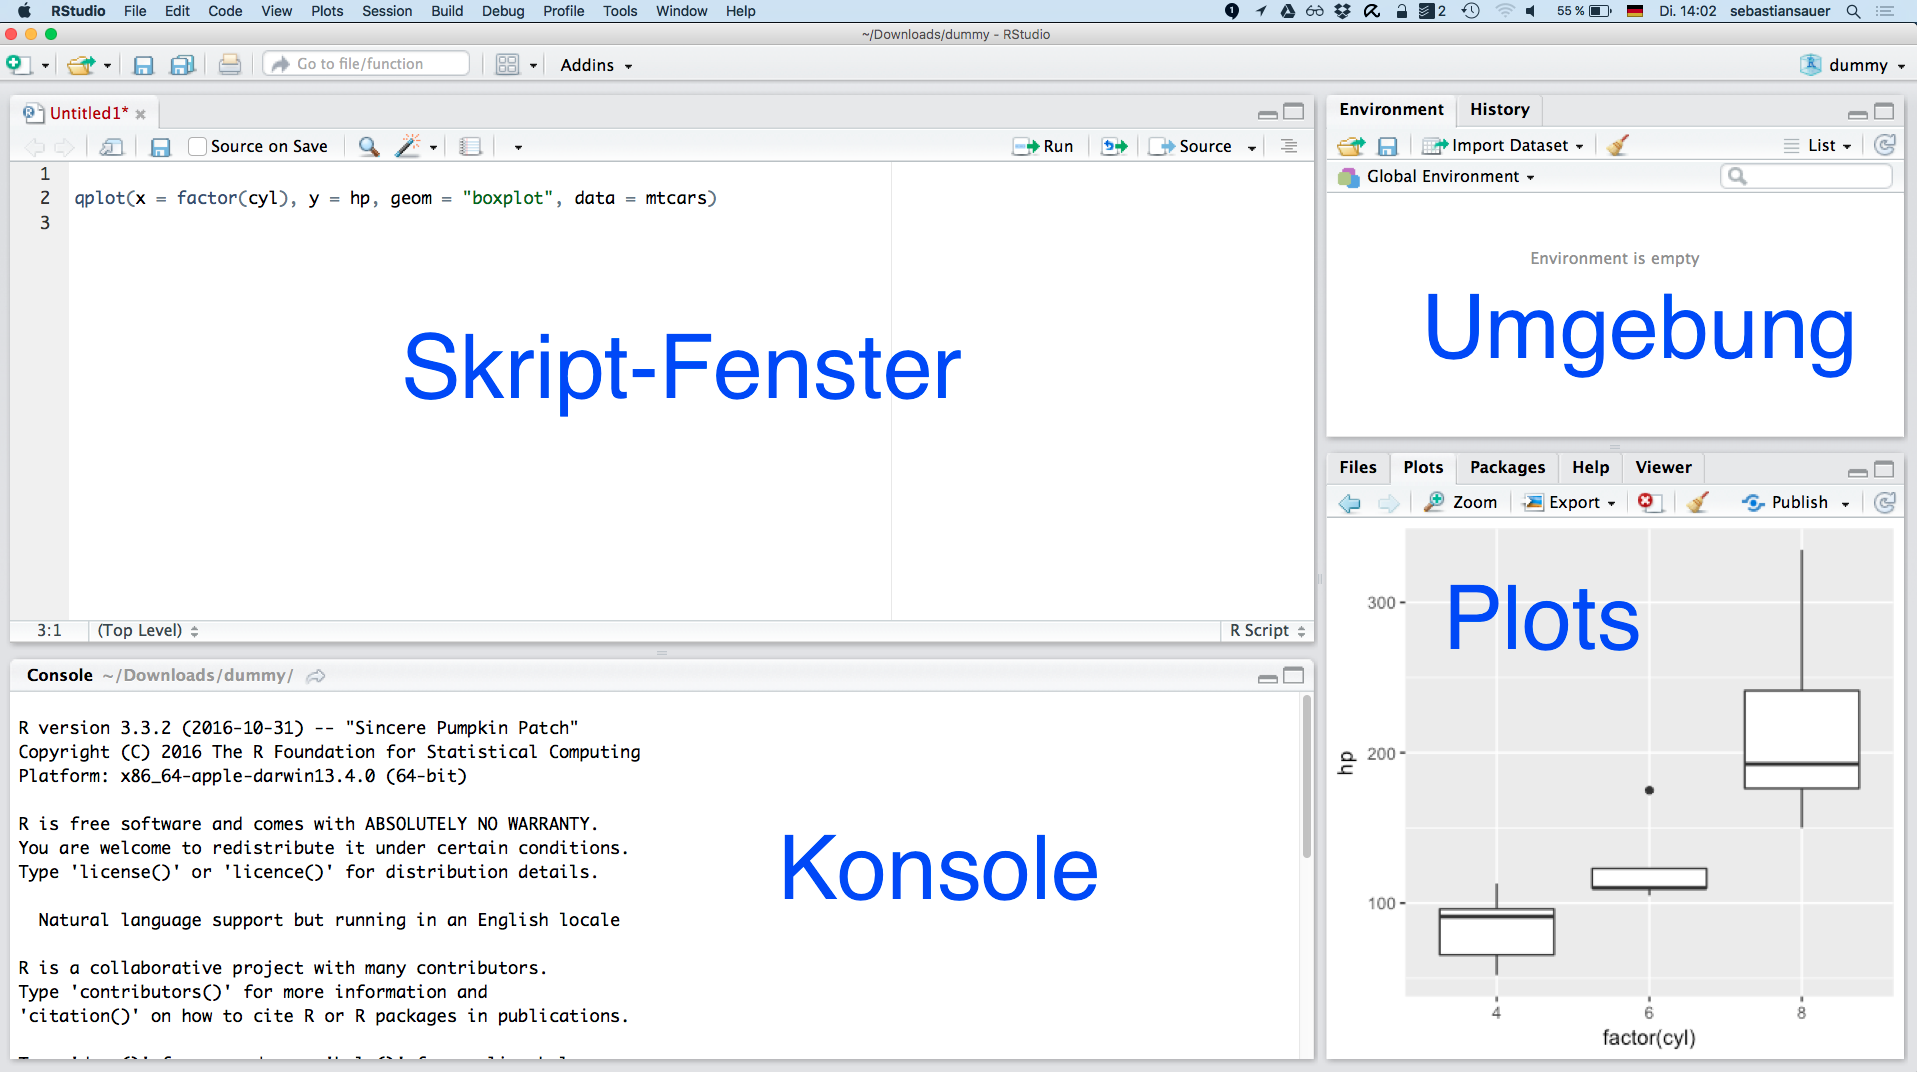
\includegraphics[width=0.7\linewidth]{./RStudioScreenshot} \end{center}

\hypertarget{erweiterungen}{%
\subsection{Erweiterungen}\label{erweiterungen}}

Außerdem brauchen wir diese Pakete für R:

\begin{itemize}
\tightlist
\item
  \texttt{tidyverse}
\item
  \texttt{mosaic}
\end{itemize}

:warning: Um einen Befehl zu verwenden, der \emph{nicht} im Standard-R,
sondern in einer Erweiterung von R (``Paket'') wohnt, müssen sie dieses
Paket erst starten (laden). Dazu können Sie den Befehl \texttt{library}
verwenden. Oder Sie klicken den Namen des Pakets hier an:

\begin{center}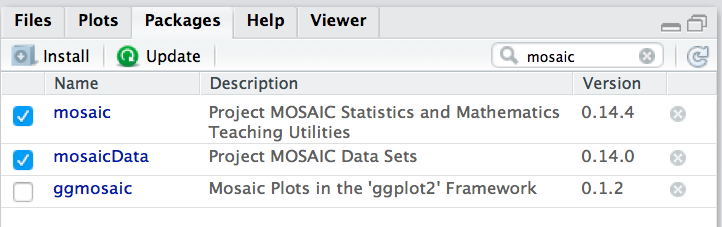
\includegraphics[width=0.7\linewidth]{https://sebastiansauer.github.io/images/2017-05-16/figure/packages_load} \end{center}

:warning: Um ein Paket zu laden, muss es installiert sein. Klicken Sie
auf den Button ``Install'' unter dem Reiter ``Packages'' in RStudio:

\begin{center}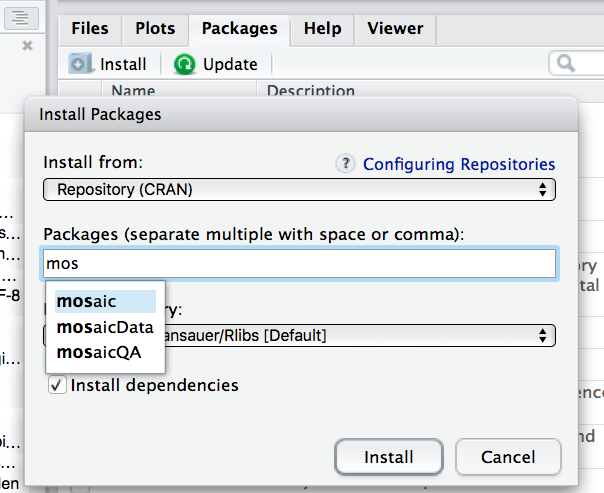
\includegraphics[width=0.7\linewidth]{https://sebastiansauer.github.io/images/2017-05-16/figure/install_packages} \end{center}

Starten Sie jetzt die beiden Erweiterungen (per Klick oder mit folgenden
Befehlen).

\begin{Shaded}
\begin{Highlighting}[]
\KeywordTok{library}\NormalTok{(mosaic)}
\KeywordTok{library}\NormalTok{(tidyverse)}
\end{Highlighting}
\end{Shaded}

\hypertarget{uber-sieben-brucken-musst-du-gehen}{%
\section{Über sieben Brücken musst Du
gehen}\label{uber-sieben-brucken-musst-du-gehen}}

\begin{center}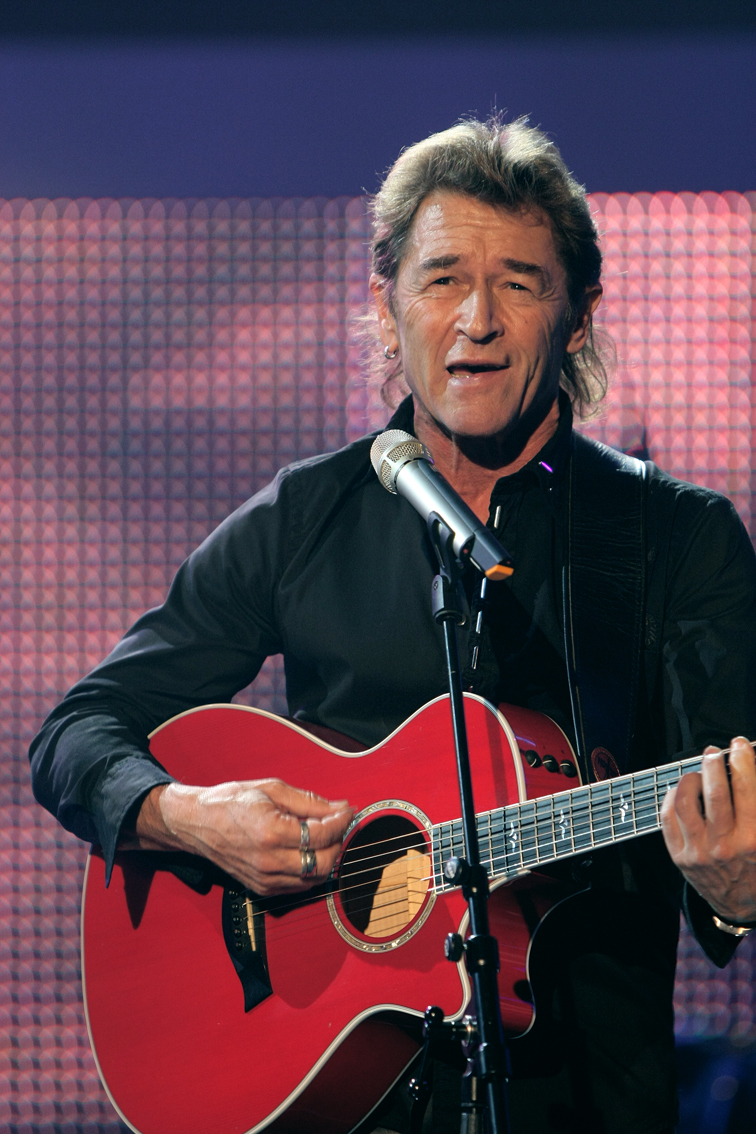
\includegraphics[width=0.3\linewidth]{https://sebastiansauer.github.io/images/2017-05-16/figure/Peter_Maffay} \end{center}

Bildlizenz: André D Conrad, CC BY SA 3.0 De,
\url{https://de.wikipedia.org/wiki/Peter_Maffay\#/media/File:Peter_Maffay.jpg}

Man kann (wenn man will) die Datenanalyse in \sout{sieben} fünf Brücken
oder Schritte einteilen, angelehnt dem Song von Peter Maffay ``Über
sieben Brücken musst du gehen''.

\begin{center}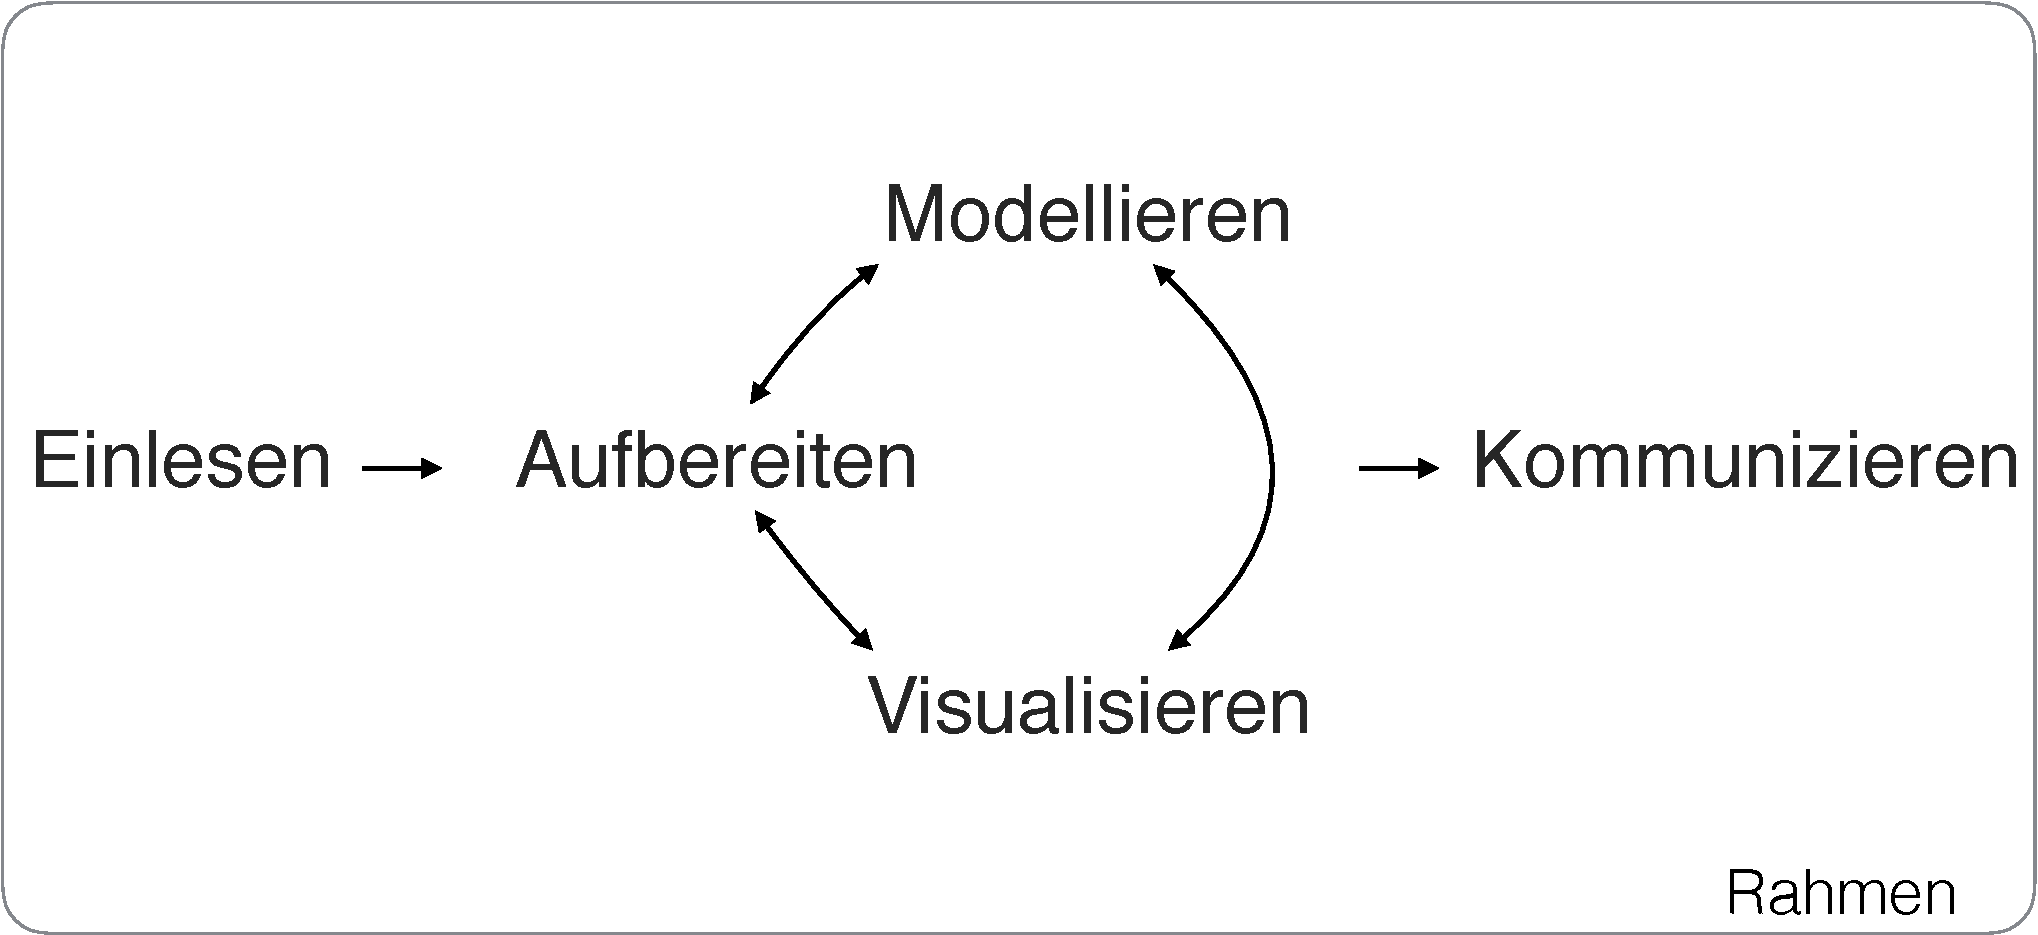
\includegraphics[width=0.7\linewidth]{https://sebastiansauer.github.io/images/2017-05-16/figure/Prozess} \end{center}

\hypertarget{brucke-1-daten-einlesen}{%
\section{Brücke 1: Daten einlesen}\label{brucke-1-daten-einlesen}}

Der einfachste Weg, Daten einzulesen, ist über den Button ``Import
Dataset'' in RStudio.

\begin{center}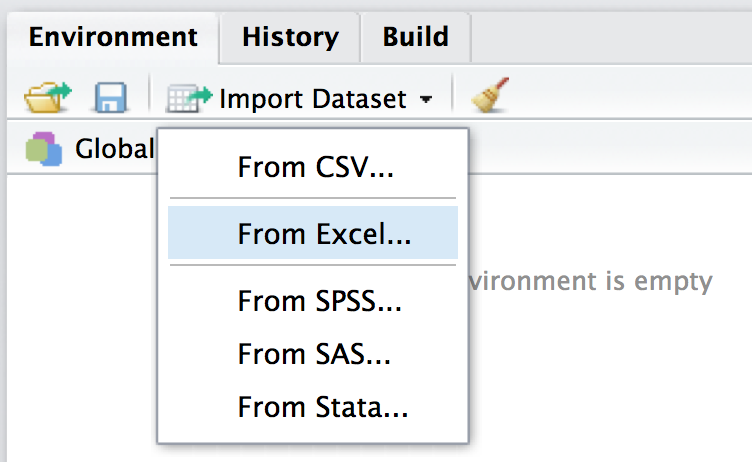
\includegraphics[width=0.7\linewidth]{https://sebastiansauer.github.io/images/2017-05-16/figure/import_RStudio} \end{center}

So lassen sich verschiedene Formate - wie XLS(X) oder CSV - importieren.

:warning: Beim Importieren von CSV-Dateien ist zu beachten, dass R davon
von \emph{us-amerikanisch} formatierten CSV-Dateien ausgeht. Was heißt
das? Das bedeutet, das Spaltentrennzeichen (delimiter) ist ein Kommma
\texttt{,}. \emph{Deutsch} formatierte CSV-Dateien, wie sie ein
deutsch-eingestellltes Excel ausgibt, nutzen aber ein Semikolon
\texttt{;} (Strichpunkt) als Spaltentrennzeichen.

Ggf. müssen Sie also in der Import-Maske von RStudio als
\emph{delimiter} ein \emph{semicolon} auswählen.

\begin{center}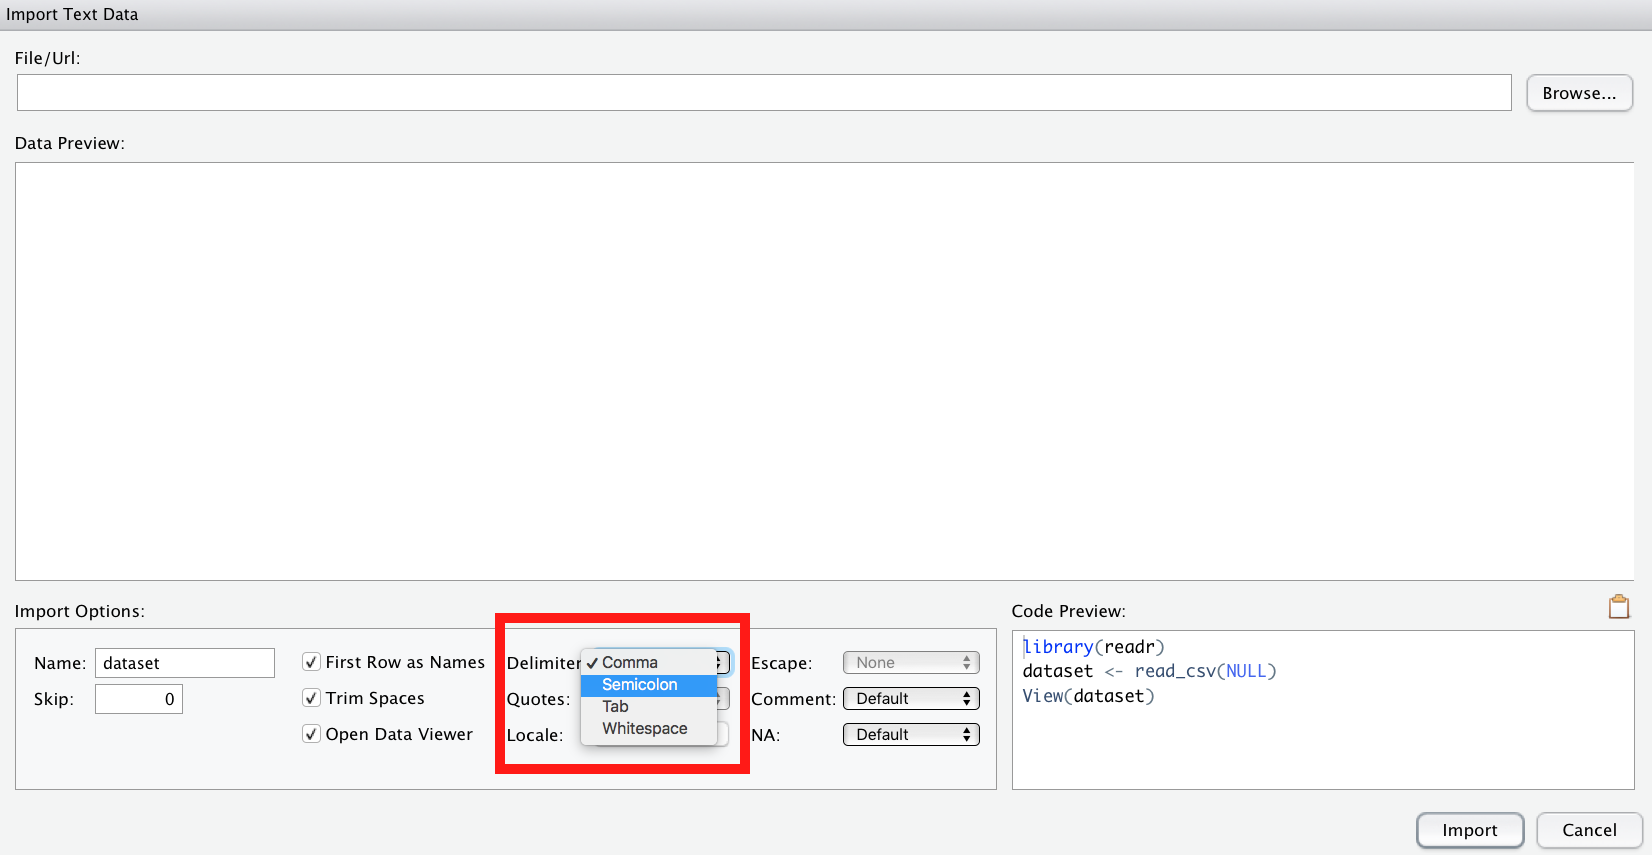
\includegraphics[width=0.7\linewidth]{https://sebastiansauer.github.io/images/2017-05-16/figure/delimiter} \end{center}

Alternativ können Sie natürlich eine XLS- oder XLSX-Datei importieren.

:bulb: Am einfachsten ist es, XLSX-Dateien zu importieren.

\hypertarget{tidy-data---tabellen-in-normalform}{%
\subsection{tidy data - Tabellen in
Normalform}\label{tidy-data---tabellen-in-normalform}}

Damit Sie in R vernünftig mit Ihren Daten arbeiten können, sollten die
Daten ``tidy'' sein, d.h. in Normalform. Was ist Normalform? Betrachten
Sie folgende Abbildung:

\begin{center}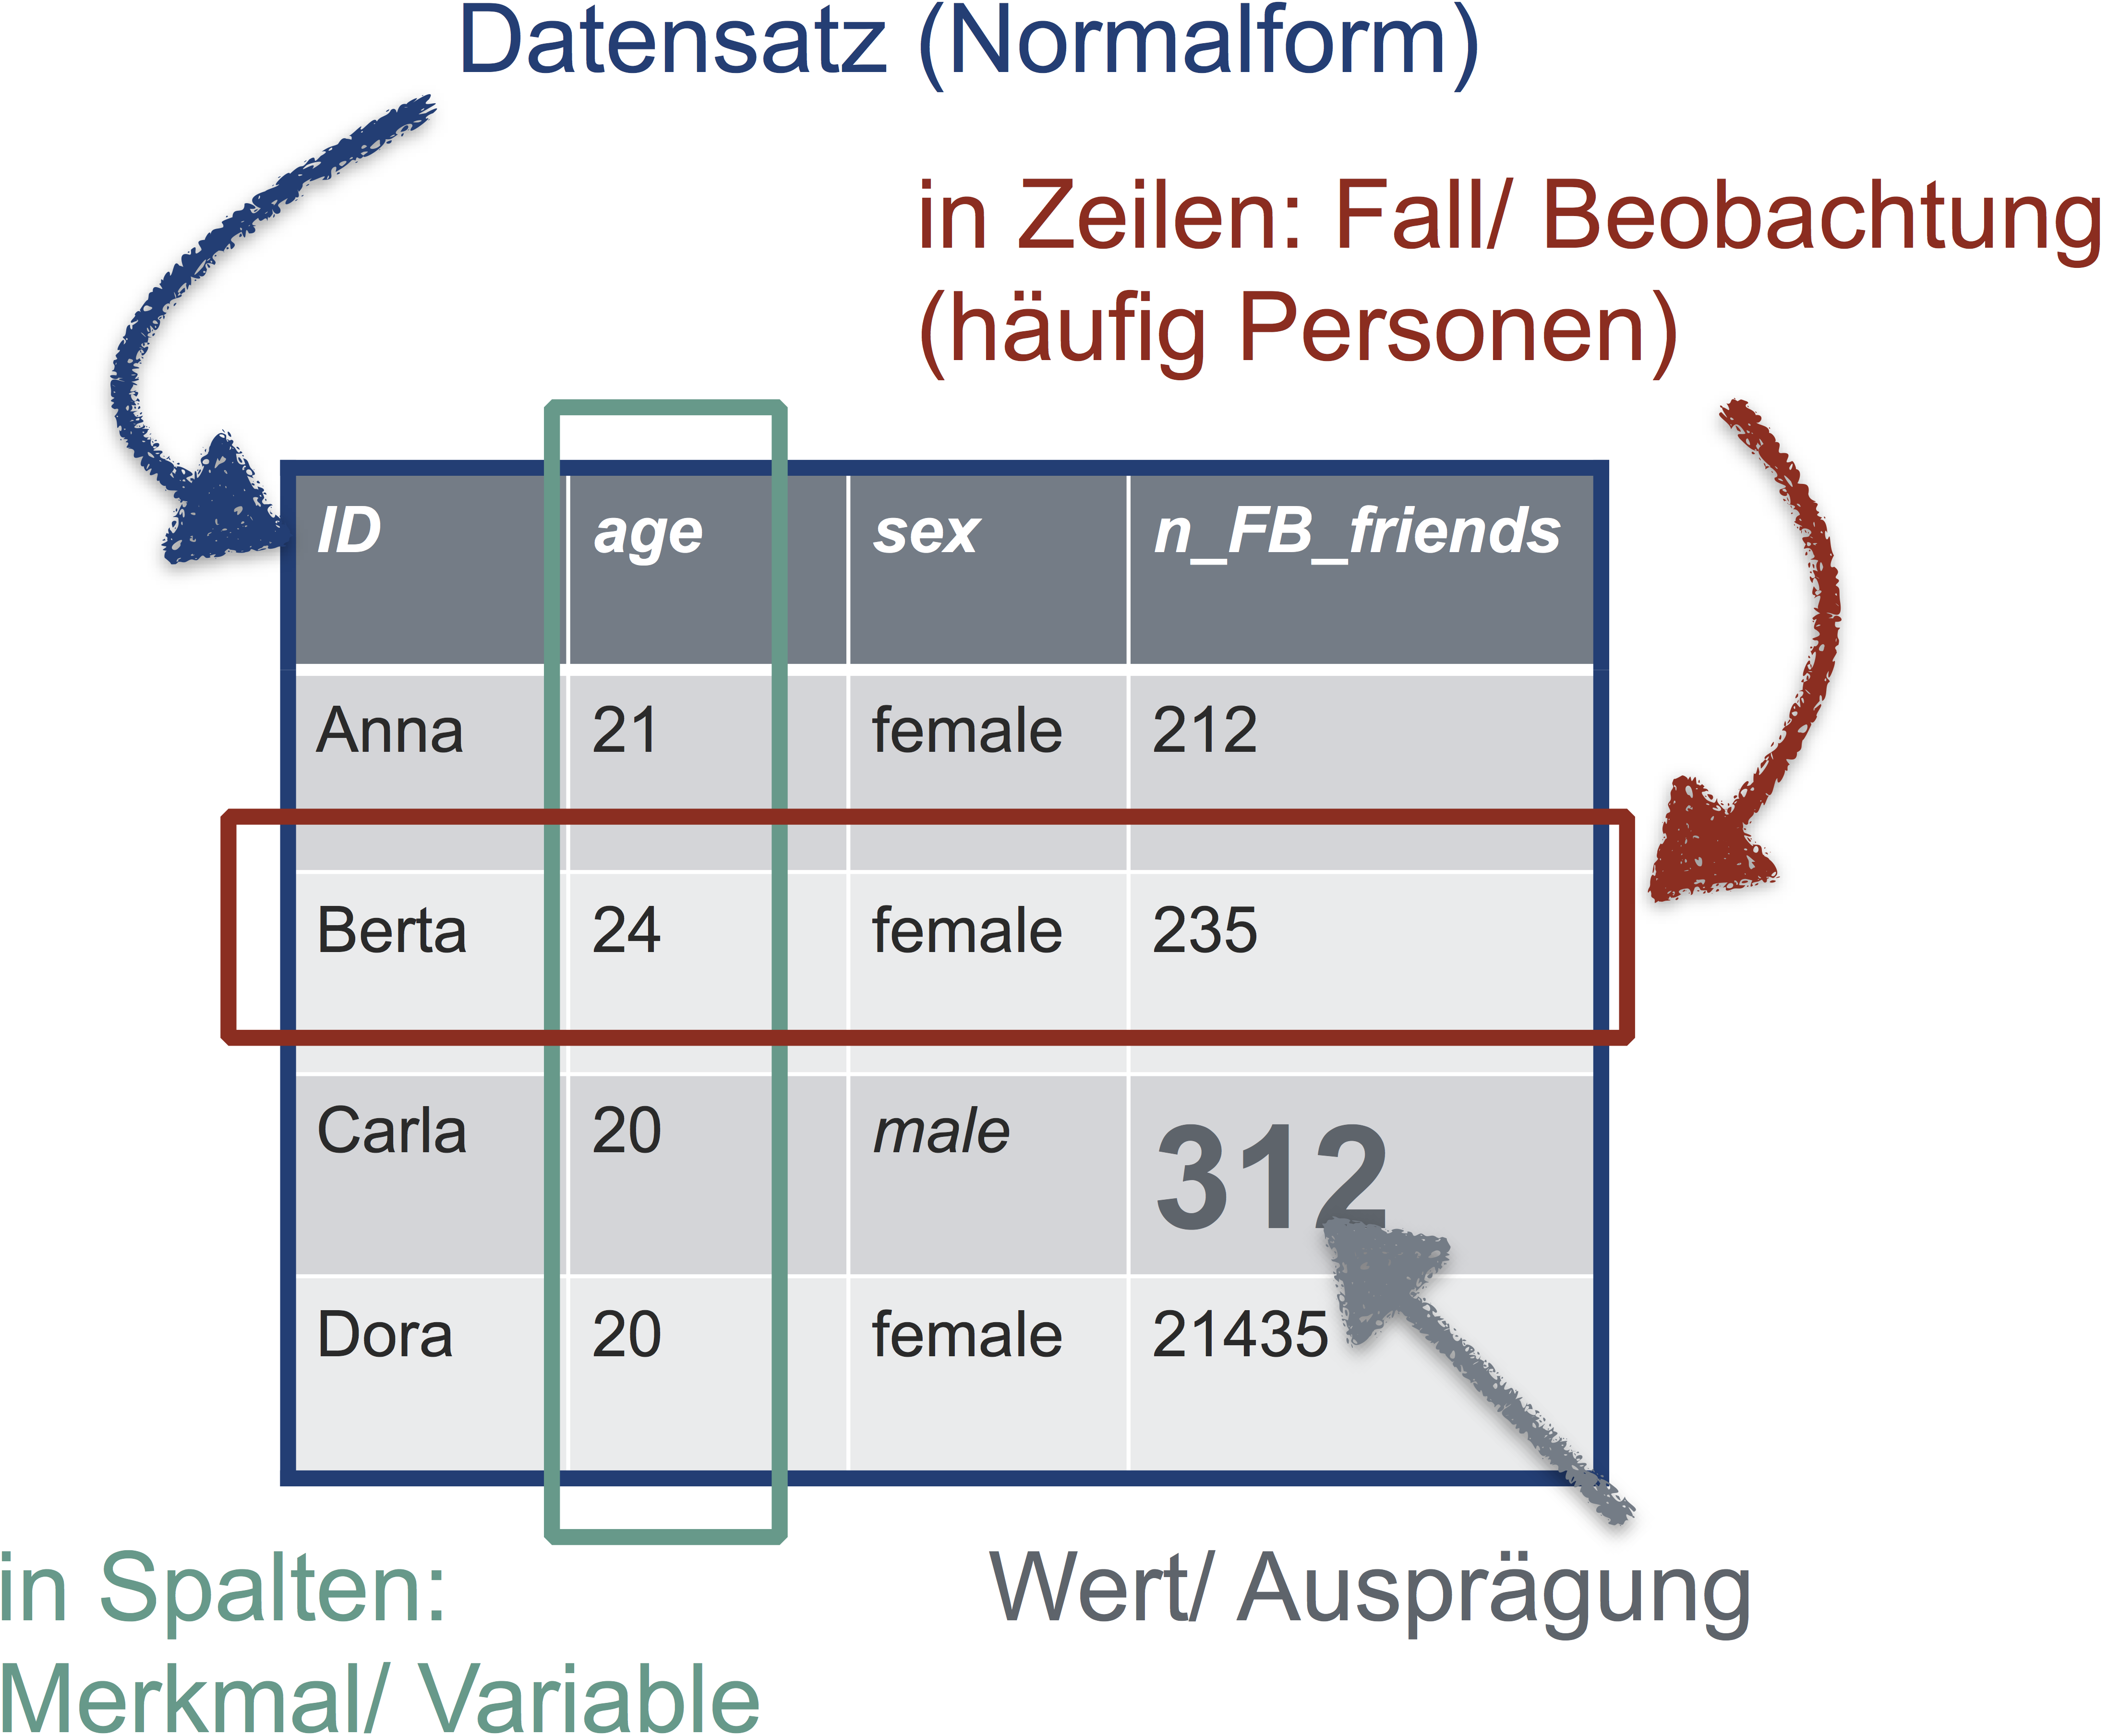
\includegraphics[width=0.7\linewidth]{https://sebastiansauer.github.io/images/2017-05-16/figure/Normalform} \end{center}

Die goldene Regel der Normalform einer Tabelle lautet also:

\begin{quote}
In jeder Zeile steht eine Beobachtung (z.B. Person). In jeder Spalte
eine Variable (z.B. Geschlecht). In der ersten Zeile stehen die
Spaltennamen, danach folgen die Werte. Sonst steht nichts in der
Tabelle.
\end{quote}

:warning: Falls Ihre Daten \emph{nicht} in Normalform sind, sollten Sie
diese zunächst in Normalform bringen.

:bulb: Der einfachste Weg (von der Lernkurve her betrachtet, nicht vom
Zeitaufwand), Daten in Normalform zu bringen, ist sie in Excel passend
umzubauen.

\hypertarget{beispiel-fur-daten-in-nicht-normalform}{%
\subsection{Beispiel für Daten in
Nicht-Normalform}\label{beispiel-fur-daten-in-nicht-normalform}}

Sie denken, dass Ihre Daten immer/auf jeden Fall in Normalform sind?
Dann scheuen Sie sich mal dieses Bild an:

\begin{center}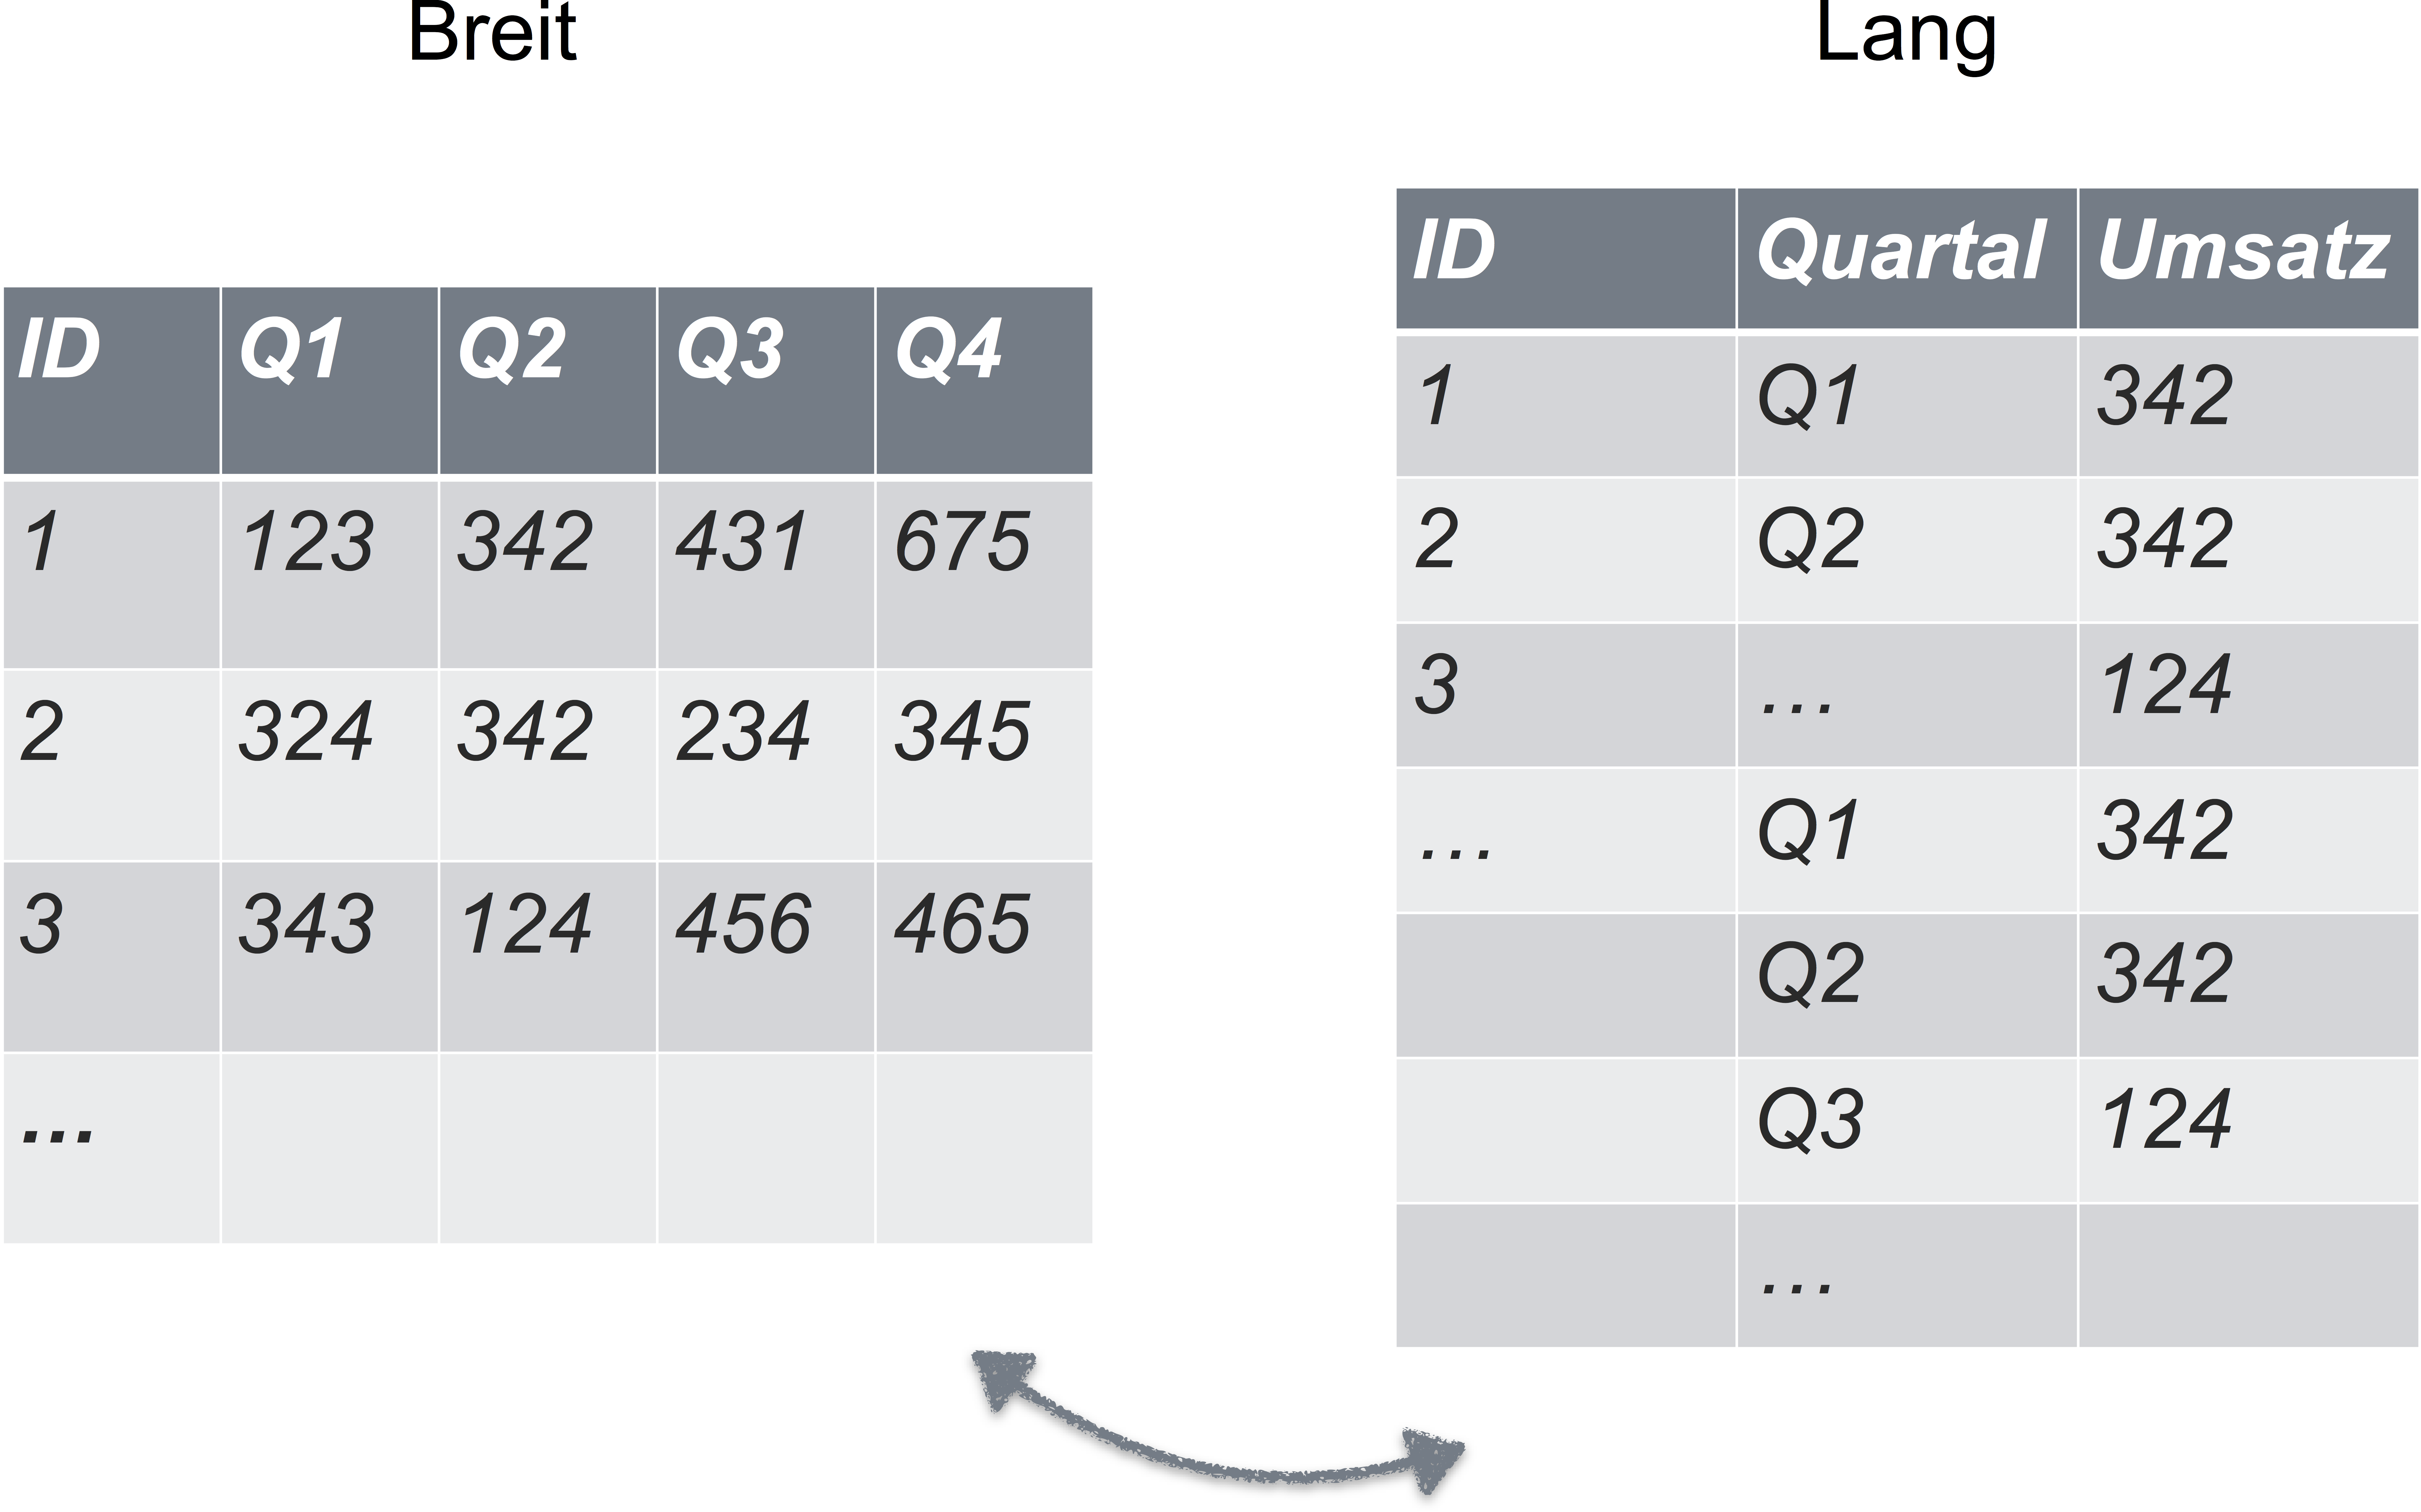
\includegraphics[width=0.7\linewidth]{https://sebastiansauer.github.io/images/2017-05-16/figure/breit_lang} \end{center}

\hypertarget{textkodierung-in-utf-8}{%
\subsection{Textkodierung in UTF-8}\label{textkodierung-in-utf-8}}

Falls Sie RStudio oder ein beliebiger Texteditor irgendwann fragt, wie
die Textdatei kodiert sein soll, wählen Sie immer ``UTF-8''. Googeln Sie
bei Interesse, was da bedeutet.

\hypertarget{schritt-2-aufbereiten}{%
\section{Schritt 2: Aufbereiten}\label{schritt-2-aufbereiten}}

Der Schritt des Aufbereitens ist häufig der zeitintensivste Schritt. In
diesem Schritt erledigen Sie alles, bevor Sie zu den ``coolen'' oder
fortgeschrittenen Analysen kommen. Z.B.

\begin{itemize}
\tightlist
\item
  prüfen auf Fehler beim Daten einlesen (und korrigieren)
\item
  Spaltennamen korrigieren
\item
  Daten umkodieren
\item
  Fehlende Werte verarzten
\item
  Komische Werte prüfen
\item
  Daten zusammenfassen
\item
  Zeilenmittelwerte bilden
\item
  Logische Variablen bilden
\end{itemize}

\hypertarget{auf-fehler-prufen}{%
\subsection{Auf Fehler prüfen}\label{auf-fehler-prufen}}

:warning: Ein häufiger Fehler ist, dass die Daten nicht richtig
eingelesen werden. Zum Beispiel werden die Spaltentrennzeichen nicht
richtig erkannt. Das kann dann so aussehen.

\begin{center}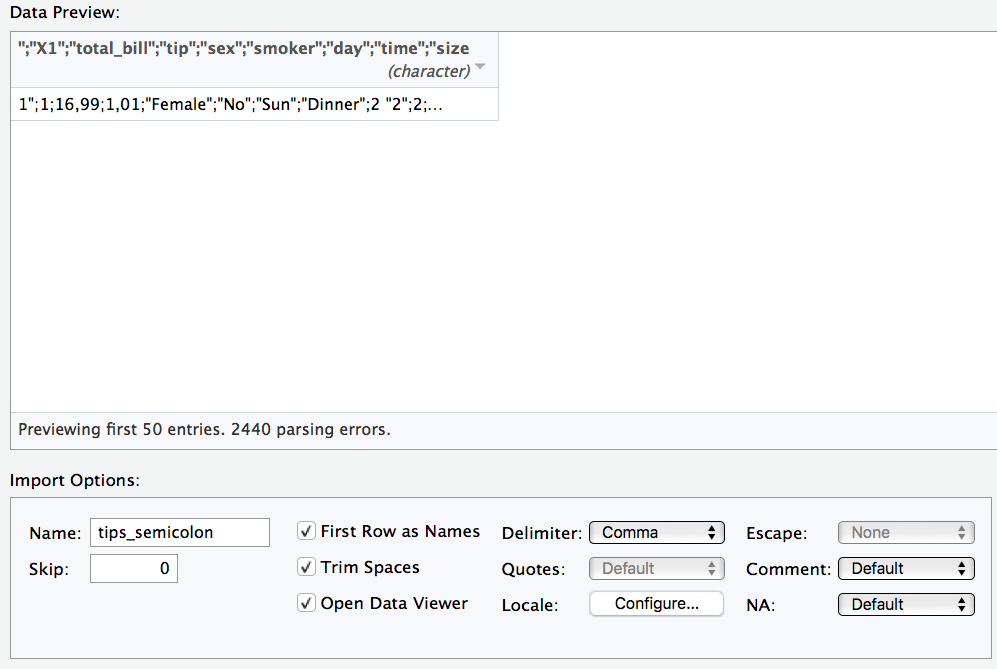
\includegraphics[width=0.7\linewidth]{https://sebastiansauer.github.io/images/2017-05-16/figure/delimiter_wrong} \end{center}

Unter ``delimiter'' in der Maske können Sie das Trennzeichen anpassen.

:warning: ``Deutsche'' CSV-Dateien verwenden als
\emph{Dezimaltrennzeichen} ein Komma; englisch-formatierte CSV-Dateien
hingegen einen Punk. R geht per Default von englisch-formatierten
CSV-Dateien aus. Importieren Sie eine deutsch-formatierte CSV-Datei,
müssen Sie das Dezimaltrennzeichen von Hand ändern; es wird nicht
automatisch erkannt.

:bulb: Unter ``locale'' können Sie das Dezimaltrennzeichen anpassen.

\hypertarget{spaltennamen-korrigieren}{%
\subsection{Spaltennamen korrigieren}\label{spaltennamen-korrigieren}}

Spaltennamen müssen auch ``tidy'' sein. Das heißt in diesem Fall:

\begin{itemize}
\tightlist
\item
  keine Leerzeichen
\item
  keine Sonderzeichen (\#,ß,ä,\ldots{})
\item
  nicht zu lang, aber trotzdem informativ
\end{itemize}

\begin{quote}
Spaltennamen sollten nur Buchstaben (ohne Umlaute) und Ziffern
enthalten.
\end{quote}

:bulb: Für Textdaten in den Spalten sind diese Regeln auch sinnvoll.

\hypertarget{umkodieren}{%
\subsection{Umkodieren}\label{umkodieren}}

Gerade bei der Analyse von Fragebogendaten ist es immer wieder nötig,
Daten umzukodieren. Klassisches Besispiel: Ein Item ist negativ kodiert.
Zum Beispiel das Item ``Ich bin ein Couch-Potato'' in einem Fragebogen
für Extraversion.

Nehmen wir an, das Item ``i04'' hat die Werte 1 (``stimme überhaupt
nicht zu'') bis 4 (``stimme voll und ganz zu''). Kreuzt jemand das
Couch-Potato-Item mit 4 an, so sollte er nicht die maximale
Extraversion-Punktzahl (4), sondern die \emph{minimale}
Extraversion-Punktzahl (1) erhalten. Also

\texttt{1\ -\/-\textgreater{}\ 4\ 2\ -\/-\textgreater{}\ 3\ 3\ -\/-\textgreater{}\ 2\ 4\ -\/-\textgreater{}\ 1}

Am einfachsten ist dies zu bewerkstelligen mit folgendem R-Befehl:

\begin{verbatim}
meine_tabelle$i04_r <- 5 - meine_Tabelle$i04
\end{verbatim}

Rechnet man \texttt{5-i04} so kommt der richtige, ``neue'' Wert heraus.

Zur Erinnerung:

\begin{itemize}
\tightlist
\item
  \texttt{\$} ist das Trennzeichen zwischen Tabellennamen und
  Spaltenname.
\item
  \texttt{\textless{}-} ist der Zuweisungsbefehl. Wir definieren eine
  neue Spalte mit dem Namen \texttt{i04\_r}. Das \texttt{r} soll stehen
  für ``rekodiert'', damit wir wissen, dass in dieser Spalte die
  umkodierten Werte stehen.
\end{itemize}

\hypertarget{fehlende-werte}{%
\subsection{Fehlende Werte}\label{fehlende-werte}}

Der einfachste Umgang mit fehlenden Werten ist: nichts machen. Denken
Sie nur daran, dass viele R-Befehle von Natur aus nervös sind - beim
Anblick von fehlenden Werten werden sie panisch und machen nix mehr. Zum
Beispiel der Befehl \texttt{mean}. Haben sie fehlende Werte in ihren
Daten, so verwenden Sie den Parameter \texttt{na.rm\ =\ TRUE}.
\texttt{na} steht für ``not available'', also fehlende Werte.
\texttt{rm} steht für ``remove''. Also
\texttt{mean(meine\_tabelle\$i04\_r,\ na.rm\ =\ TRUE)}.

:bulb: Der R-Befehl \texttt{summary} zeigt Ihnen an, ob es fehlende
Werte gibt:

\texttt{summary(meine\_daten)}.

\hypertarget{komische-werte}{%
\subsection{Komische Werte}\label{komische-werte}}

Hat ein Spaßvogel beim Alter 999 oder -1 angegeben, kann das Ihre Daten
ganz schön verhageln. Prüfen Sie die Daten auf komische Werte. Der
einfachste Weg ist, sich die Daten in Excel anzuschauen. Cleverer ist
noch, sich Zusammenfassungen auszugeben, wie der kleinste oder der
größte Wert, oder der Mittelwert etc., und dann zu schauen, ob einem
etwas spanisch vorkommt. Diagramme sind ebenfalls hilfreich.

\hypertarget{logische-variablen-bilden}{%
\subsection{Logische Variablen bilden}\label{logische-variablen-bilden}}

Sagen wir, uns interessiert welches Auto mehr als 200 PS hat; wir wollen
Autos mit mehr als 200 PS vergleichen (``Spass'') mit schwach
motorisierten Autos (``Kruecke''). Wie können wir das (einfach) in R
erreichen? Logische Variablen sind ein einfacher Weg.

\begin{Shaded}
\begin{Highlighting}[]
\NormalTok{mtcars}\OperatorTok{$}\NormalTok{Spass <-}\StringTok{ }\NormalTok{mtcars}\OperatorTok{$}\NormalTok{hp }\OperatorTok{>}\StringTok{ }\DecValTok{200}
\end{Highlighting}
\end{Shaded}

Dieser Befehl hat eine Spalte (Variable) in der Tabelle \texttt{mtcars}
erzeugt, in der \texttt{TRUE} steht, wenn das Auto der jeweiligen Spalte
die Bedingung (hp \textgreater{} 200) erfüllt. Schauen Sie nach.

\begin{Shaded}
\begin{Highlighting}[]
\KeywordTok{favstats}\NormalTok{(mtcars}\OperatorTok{$}\NormalTok{Spass)}
\end{Highlighting}
\end{Shaded}

\begin{verbatim}
## Warning in fav_stats(x, ..., na.rm = na.rm): Auto-converting logical to
## numeric.
\end{verbatim}

\begin{verbatim}
##  min Q1 median Q3 max    mean        sd  n missing
##    0  0      0  0   1 0.21875 0.4200134 32       0
\end{verbatim}

\hypertarget{daten-zusammenfassen-deskriptivstatistik}{%
\subsection{Daten zusammenfassen:
Deskriptivstatistik}\label{daten-zusammenfassen-deskriptivstatistik}}

Deskriptive Statistik ist letztlich nichts anderes, als Daten geschickt
zusammenzufassen.

\begin{quote}
Praktisch sind es meistens Spalten, die zu einen Zahl zusammengefasst
werden.
\end{quote}

\begin{center}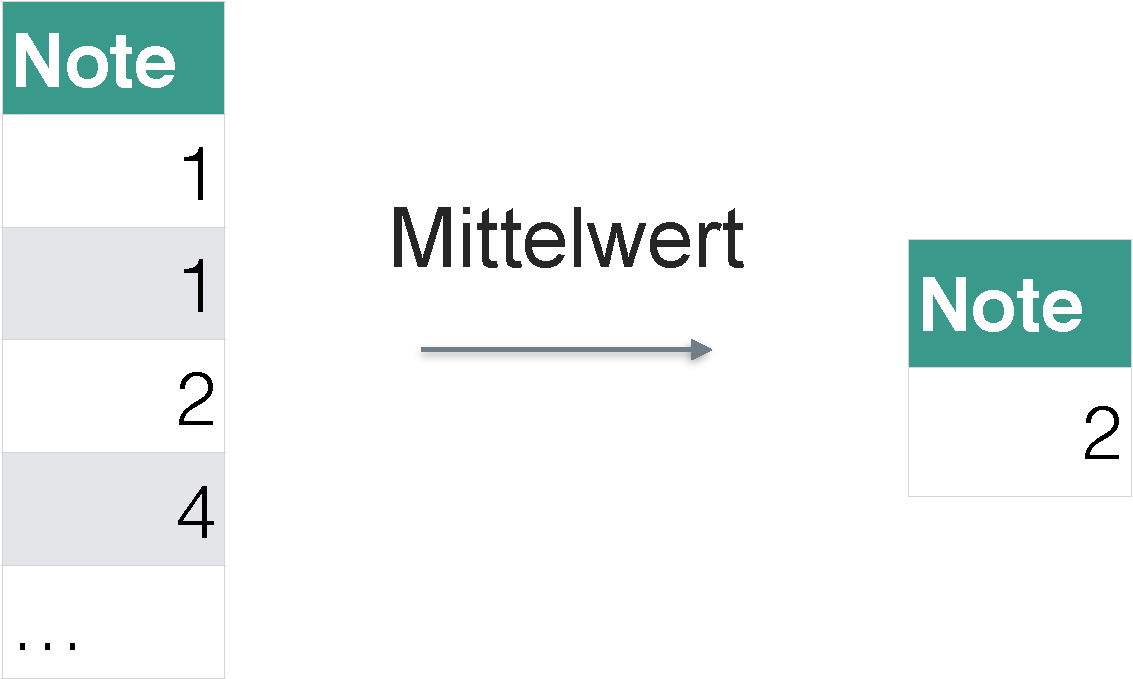
\includegraphics[width=0.7\linewidth]{https://sebastiansauer.github.io/images/2017-05-16/figure/summarise} \end{center}

Schauen wir uns das mal mit echten Daten an. Der Datensatz ``mtcars''
ist schon in R eingebaut, so dass wir in nicht extra laden müssen. Ganz
praktisch.

\begin{Shaded}
\begin{Highlighting}[]
\KeywordTok{summary}\NormalTok{(mtcars)}
\end{Highlighting}
\end{Shaded}

\begin{verbatim}
##       mpg             cyl             disp             hp       
##  Min.   :10.40   Min.   :4.000   Min.   : 71.1   Min.   : 52.0  
##  1st Qu.:15.43   1st Qu.:4.000   1st Qu.:120.8   1st Qu.: 96.5  
##  Median :19.20   Median :6.000   Median :196.3   Median :123.0  
##  Mean   :20.09   Mean   :6.188   Mean   :230.7   Mean   :146.7  
##  3rd Qu.:22.80   3rd Qu.:8.000   3rd Qu.:326.0   3rd Qu.:180.0  
##  Max.   :33.90   Max.   :8.000   Max.   :472.0   Max.   :335.0  
##       drat             wt             qsec             vs        
##  Min.   :2.760   Min.   :1.513   Min.   :14.50   Min.   :0.0000  
##  1st Qu.:3.080   1st Qu.:2.581   1st Qu.:16.89   1st Qu.:0.0000  
##  Median :3.695   Median :3.325   Median :17.71   Median :0.0000  
##  Mean   :3.597   Mean   :3.217   Mean   :17.85   Mean   :0.4375  
##  3rd Qu.:3.920   3rd Qu.:3.610   3rd Qu.:18.90   3rd Qu.:1.0000  
##  Max.   :4.930   Max.   :5.424   Max.   :22.90   Max.   :1.0000  
##        am              gear            carb         Spass         cyl_f 
##  Min.   :0.0000   Min.   :3.000   Min.   :1.000   Mode :logical   4:11  
##  1st Qu.:0.0000   1st Qu.:3.000   1st Qu.:2.000   FALSE:25        6: 7  
##  Median :0.0000   Median :4.000   Median :2.000   TRUE :7         8:14  
##  Mean   :0.4062   Mean   :3.688   Mean   :2.812   NA's :0               
##  3rd Qu.:1.0000   3rd Qu.:4.000   3rd Qu.:4.000                         
##  Max.   :1.0000   Max.   :5.000   Max.   :8.000
\end{verbatim}

Hilfe zu diesem Datensatz bekommen Sie so:

\begin{Shaded}
\begin{Highlighting}[]
\KeywordTok{help}\NormalTok{(mtcars)}
\end{Highlighting}
\end{Shaded}

:bulb: mit \texttt{help(Befehl)} bekommt man Hilfe zu einem Befehl oder
einem sonstigen Objekt (z.B. Datensatz).

\hypertarget{numerische-variablen}{%
\subsubsection{Numerische Variablen}\label{numerische-variablen}}

Der einfachste Weg, um Deskriptivstatistik für eine \emph{numerische
Variable} auf einen Abwasch zu erledigen ist dieser Befehl:

\begin{Shaded}
\begin{Highlighting}[]
\KeywordTok{favstats}\NormalTok{(mtcars}\OperatorTok{$}\NormalTok{mpg)}
\end{Highlighting}
\end{Shaded}

\begin{verbatim}
##   min     Q1 median   Q3  max     mean       sd  n missing
##  10.4 15.425   19.2 22.8 33.9 20.09062 6.026948 32       0
\end{verbatim}

Der Befehl \texttt{favstats} lässt auch Subgruppenanalysen zu, z.B. um
Männer und Frauen zu vergleichen:

\begin{Shaded}
\begin{Highlighting}[]
\KeywordTok{favstats}\NormalTok{(mpg }\OperatorTok{~}\StringTok{ }\NormalTok{cyl, }\DataTypeTok{data =}\NormalTok{ mtcars)}
\end{Highlighting}
\end{Shaded}

\begin{verbatim}
##   cyl  min    Q1 median    Q3  max     mean       sd  n missing
## 1   4 21.4 22.80   26.0 30.40 33.9 26.66364 4.509828 11       0
## 2   6 17.8 18.65   19.7 21.00 21.4 19.74286 1.453567  7       0
## 3   8 10.4 14.40   15.2 16.25 19.2 15.10000 2.560048 14       0
\end{verbatim}

Dabei ist \texttt{mpg} die Variable, die sie vergleichen wollen
(Spritverbrauch); \texttt{cyl} die Gruppierungsvariable (Anzahl der
Zylinder). Gruppierungsvariable bedeutet hier, dass den Spritverbrauch
zwischen 4,6 und 8-Zylindern vergleichen wollen.

\hypertarget{nominale-variablen}{%
\subsubsection{Nominale Variablen}\label{nominale-variablen}}

Eine Häufigkeitstabelle für eine \emph{nicht-metrische} Variable lässt
über den Befehl \texttt{table} erstellen.

Aber zuerst wandeln wir eine unserer metrischen Variablen in eine
nominale um:

\begin{Shaded}
\begin{Highlighting}[]
\NormalTok{my_cars <-}\StringTok{ }\NormalTok{mtcars}

\NormalTok{my_cars}\OperatorTok{$}\NormalTok{cyl_f <-}\StringTok{ }\KeywordTok{factor}\NormalTok{(mtcars}\OperatorTok{$}\NormalTok{cyl)}
\NormalTok{my_cars}\OperatorTok{$}\NormalTok{Spass <-}\StringTok{ }\NormalTok{my_cars}\OperatorTok{$}\NormalTok{hp }\OperatorTok{>}\StringTok{ }\DecValTok{200}
\end{Highlighting}
\end{Shaded}

\texttt{factor} wandelt eine metrische (numerische) Variable in einen
nominale Variable um; nominale Variablen nennt man in R auch ``Faktor''.
Um den ``originalen'' Datensatz nicht zu überschreiben, packen wir alles
in eine Kopie mit dem Namen \texttt{my\_cars}.

\begin{Shaded}
\begin{Highlighting}[]
\KeywordTok{table}\NormalTok{(my_cars}\OperatorTok{$}\NormalTok{cyl_f)}
\end{Highlighting}
\end{Shaded}

\begin{verbatim}
## 
##  4  6  8 
## 11  7 14
\end{verbatim}

Aha, 14 Autos in unserer Tabelle haben also 8 Zylinder.

Brechen wir jetzt die Auszählunng noch mal auf in ``Spass'' vs.
``Krücke''.

\begin{Shaded}
\begin{Highlighting}[]
\KeywordTok{table}\NormalTok{(my_cars}\OperatorTok{$}\NormalTok{cyl_f, my_cars}\OperatorTok{$}\NormalTok{Spass)}
\end{Highlighting}
\end{Shaded}

\begin{verbatim}
##    
##     FALSE TRUE
##   4    11    0
##   6     7    0
##   8     7    7
\end{verbatim}

\hypertarget{zeilenmittelwerte-bilden}{%
\subsection{Zeilenmittelwerte bilden}\label{zeilenmittelwerte-bilden}}

Bei Umfragen kommt es häufig vor, dass man Zeilenmittelwerte bildet.
Wieso? Man möchte z.B. in einer Mitarbeiterbefragung den
``Engagementwert'' jedes Beschäftigten wissen (klingt einfach gut). Dazu
addiert man die Werte jedes passenden Items auf. Diese Summe teilen Sie
durch die Anzahl der Spalten

:bulb: Zeilenmittelwerte bilden Sie am einfachsten in Excel.

In R können Sie Zeilen einfach mit dem \texttt{+} Zeichen addieren:

\begin{verbatim}
meine_tabelle$zeilenmittelwert <- (meine_tabelle$item1 + meine Tabelle$item2) / 2
\end{verbatim}

\hypertarget{schritt-3-visualisieren}{%
\section{Schritt 3: Visualisieren}\label{schritt-3-visualisieren}}

Ein Bild sagt bekanntlich mehr als 1000 Worte. Betrachten Sie dazu
``Anscombes Quartett'':

\begin{center}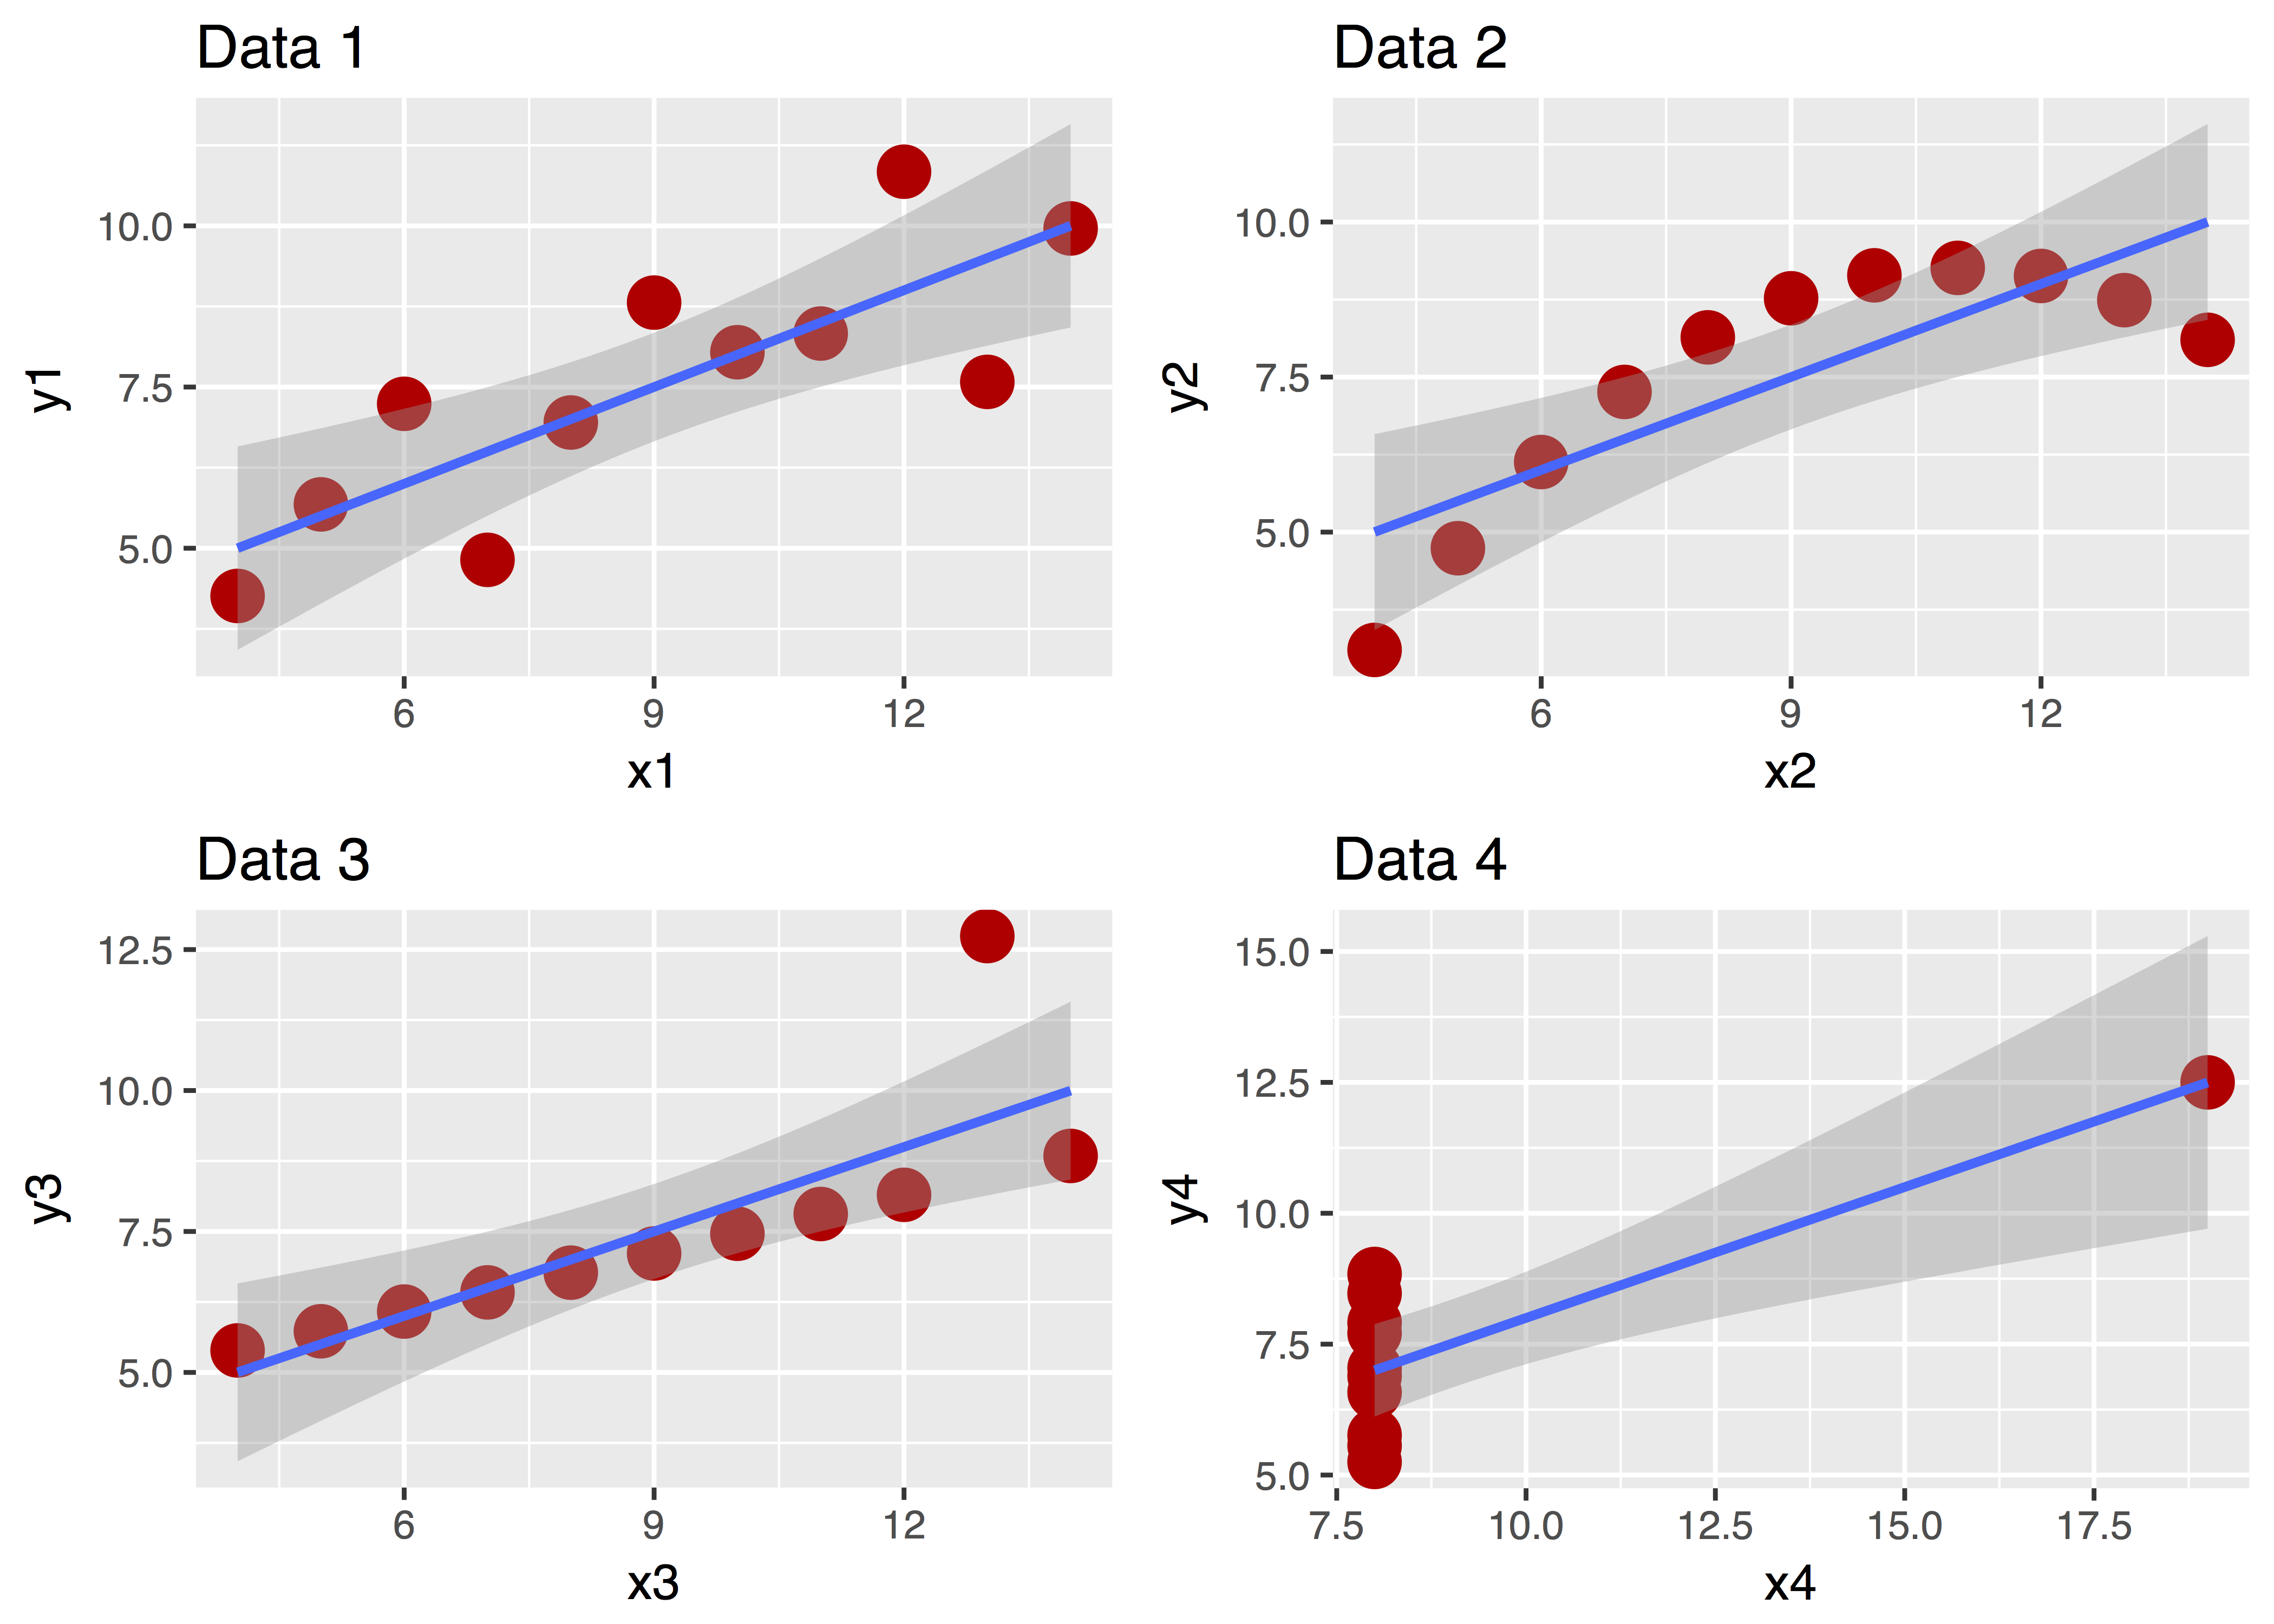
\includegraphics[width=0.7\linewidth]{https://sebastiansauer.github.io/images/2017-05-16/figure/anscombe} \end{center}

Diese vier Datensätze sehen ganz unterschiedlich aus, nicht wahr? Aber
ihre zentralen deskriptiven Statistiken sind praktisch gleich! Ohne
Diagramm wäre uns diese Unterschiedlichkeit nicht (so leicht)
aufgefallen!

Zur Visualisierung empfehle ich das R-Paket \texttt{ggplot2}. Es wird
mit geladen, wenn Sie \texttt{tidyverse} laden.

Es gib einen recht einfachen Befehl in diesem Paket, \texttt{qplot}. Bei
\texttt{qplot} geben Sie folgende Parameter an:

\begin{itemize}
\tightlist
\item
  X-Achse (\texttt{x}): Welche Variable (Spalte in ihrer Tabelle) soll
  auf der X-Achse stehen?\\
\item
  Y-Achse (\texttt{y}): Welche Variable (Spalte in ihrer Tabelle) soll
  auf der Y-Achse stehen?
\item
  Daten (\texttt{data}): Wie heißt ihre Datentabelle?
\item
  Geom (\texttt{geom}): Welche Art von Bildchen wollen Sie malen (z.B.
  Punkte, Boxplots, Linien, Histogramm\ldots{})`
\end{itemize}

Darüber hinaus verkrafter der Befehl noch viele andere Schnörkel, die
wir uns hier sparen. Interessierte können googeln\ldots{} Es ist ein
sehr mächtiger Befehl, der sehr ansprechende Diagramme erzeugen kann.

Probieren wir's!

\begin{Shaded}
\begin{Highlighting}[]
\KeywordTok{qplot}\NormalTok{(}\DataTypeTok{x =}\NormalTok{ hp,}
      \DataTypeTok{y =}\NormalTok{ mpg,}
      \DataTypeTok{geom =} \StringTok{"point"}\NormalTok{,}
      \DataTypeTok{data =}\NormalTok{ mtcars)}
\end{Highlighting}
\end{Shaded}

Easy, oder?

Ein anderes Geom:

\begin{Shaded}
\begin{Highlighting}[]
\KeywordTok{qplot}\NormalTok{(}\DataTypeTok{x =} \KeywordTok{factor}\NormalTok{(cyl),}
      \DataTypeTok{y =}\NormalTok{ mpg,}
      \DataTypeTok{data =}\NormalTok{ mtcars,}
      \DataTypeTok{geom =} \StringTok{"boxplot"}\NormalTok{)}
\end{Highlighting}
\end{Shaded}

Beachten Sie, dass \texttt{qplot} nur dann \emph{mehrere} Boxplots
zeichnet, wenn auf der X-Achse eine nominal skalierte Variable steht.

:bulb: Eine metrische Variable wandeln Sie in eine nominal skalierte
Variable um mit dem Befehl \texttt{factor(meine\_metrische\_variable)}.

Oder mal nur eine Variable:

\begin{Shaded}
\begin{Highlighting}[]
\KeywordTok{qplot}\NormalTok{(}\DataTypeTok{x =}\NormalTok{ hp,}
      \DataTypeTok{data =}\NormalTok{ mtcars,}
      \DataTypeTok{geom =} \StringTok{"histogram"}\NormalTok{)}
\end{Highlighting}
\end{Shaded}

:bulb: Geben wir keine Y-Variable an, nimmt qplot eigenständig die
Häufigkeit pro X-Wert!

:bulb: Tauschen Sie mal ``histogram'' mit ``density''!

\hypertarget{schritt-4-modellieren}{%
\section{Schritt 4: Modellieren}\label{schritt-4-modellieren}}

Modellieren hört sich kompliziert an. Für uns hier heißt es vor allem
ein inferenzstatistisches Verfahren anzuwenden.

:bulb: Das Schweizer Taschenmesser und den Modellierungsverfahren ist
die Regressionsanalyse. Man kann sie für viele Zwecke einsetzen.

\hypertarget{wann-welchen-test}{%
\subsection{Wann welchen Test?}\label{wann-welchen-test}}

Es gibt in vielen Lehrbüchern Übersichten zur Frage, wann man welchen
Test rechnen soll. Googeln hilft hier auch weiter. Eine Übersicht findet
man hier: \url{http://www.methodenberatung.uzh.ch/de/datenanalyse.html}.

\hypertarget{wie-heit-der-jeweilige-r-befehl}{%
\subsection{Wie heißt der jeweilige
R-Befehl?}\label{wie-heit-der-jeweilige-r-befehl}}

Wenn man diese Befehle nicht häufig verwendet, ist es schwierig, sie
auswändig zu wissen. Googeln Sie. Eine gute Übersicht findet sich hier:
\url{http://r-statistics.co/Statistical-Tests-in-R.html}.

\hypertarget{regression}{%
\subsection{Regression}\label{regression}}

Weil die Regression so praktisch ist, hier ein Beispiel.

\begin{Shaded}
\begin{Highlighting}[]
\KeywordTok{lm}\NormalTok{(mpg }\OperatorTok{~}\StringTok{ }\NormalTok{cyl, }\DataTypeTok{data =}\NormalTok{ mtcars)}
\end{Highlighting}
\end{Shaded}

\begin{verbatim}
## 
## Call:
## lm(formula = mpg ~ cyl, data = mtcars)
## 
## Coefficients:
## (Intercept)          cyl  
##      37.885       -2.876
\end{verbatim}

\texttt{lm} heißt ``lineares Modell'' - weil man bei der (normalen)
Regression eine Gerade in die Punktewolke der Daten legt, um den Trend
zu abzuschätzen. Als nächstes gibt man die ``Ziel-Variable'' (Output)
an, hier \texttt{mpg}. Dann kommt ein Kringel \texttt{\textasciitilde{}}
gefolgt von einer (mehr) Input-Variablen (Prädiktoren, UVs). Schließnoch
muss noch die Datentabelle erwähnt werden.

Das Ergbebnis sagt uns, dass \emph{pro Zylinder} die Variable
\texttt{mpg} um knapp 3 Punkte sinkt. Also: Hat die Karre einen Zylinder
mehr, so kann man pro Galone Sprit 3 Meilen weniger fahren. Immer im
Schnitt, versteht sich. (Und wenn die Voraussetzungen erfüllt sind, aber
darum kümmern wir uns jetzt nicht.)

Allgemein:

\begin{verbatim}
lm(output ~ input, data = meine_daten)
\end{verbatim}

Easy, oder?

Man kann auch mehrere Prädiktoren anführen:

\begin{Shaded}
\begin{Highlighting}[]
\KeywordTok{lm}\NormalTok{(mpg }\OperatorTok{~}\StringTok{ }\NormalTok{cyl }\OperatorTok{+}\StringTok{ }\NormalTok{hp, }\DataTypeTok{data =}\NormalTok{ mtcars)}
\end{Highlighting}
\end{Shaded}

\begin{verbatim}
## 
## Call:
## lm(formula = mpg ~ cyl + hp, data = mtcars)
## 
## Coefficients:
## (Intercept)          cyl           hp  
##    36.90833     -2.26469     -0.01912
\end{verbatim}

Dazu werden die durch \texttt{+} getrennt. Die Ergebnisse zeigen uns,
dass die PS-Zahl (´hp´) kaum Einfluss auf den Spritverbrauch haut.
Genauer: Kaum \emph{zusätzlichen} Einfluss auf den Spritverbrauch hat.
Also Einfluss, der über den Einfluss hinausgeht, der schon durch die
Anzahl der Zylinder erklärt werden würde. Es ist also praktisch wurscht,
wie viel PS das Auto hat, wenn man den Verbrauch schätzen will -
Hauptsache, man weiß die Anzahl der Zylinder.

\hypertarget{vorhersagen}{%
\subsection{Vorhersagen}\label{vorhersagen}}

Man kann die Regression nutzen, um Vorhersagen zu treffen. Sagen wir,
unser neuer Lamborghini hat 400 PS und 12 Zylinder. Wie groß ist wohl
der Spritverbrauch laut unserem Regressionsmodell?

Als Vorbereitung speichern wir unser Regressionsmodell in einer eigenen
Variablen:

\begin{Shaded}
\begin{Highlighting}[]
\NormalTok{mein_lm <-}\StringTok{ }\KeywordTok{lm}\NormalTok{(mpg }\OperatorTok{~}\StringTok{ }\NormalTok{cyl }\OperatorTok{+}\StringTok{ }\NormalTok{hp, }\DataTypeTok{data =}\NormalTok{ mtcars)}
\end{Highlighting}
\end{Shaded}

Dazu nimmt man am besten den Befehl \texttt{predict}, weil wir wollen
eine Vorhersage treffen:

\begin{Shaded}
\begin{Highlighting}[]
\KeywordTok{predict}\NormalTok{(mein_lm, }\KeywordTok{data.frame}\NormalTok{(}\DataTypeTok{cyl =} \DecValTok{12}\NormalTok{, }\DataTypeTok{hp =} \DecValTok{400}\NormalTok{))}
\end{Highlighting}
\end{Shaded}

\begin{verbatim}
##        1 
## 2.083329
\end{verbatim}

Aha. Pro Gallone kämmen wir 2 Meilen. Schluckspecht.

\hypertarget{visualisierung-des-modells}{%
\subsection{Visualisierung des
Modells}\label{visualisierung-des-modells}}

Schauen wir uns das Modell mal an, damit es nicht so theoretisch ist.
Wie gesagt, ein Regressionsmodell ist nichts anderes als eine
Trendgerade in einer Punktewolke.

:bulb: Gerade sind durch Achsenabschnitt (engl. ``intercept'') f(x=0)
und Steigung (englisch: ``slope'') definiert. Der Steigungswert ist die
Zahl, die der lm-Befehl für den Prädiktor ausspuckt

\begin{Shaded}
\begin{Highlighting}[]
\KeywordTok{qplot}\NormalTok{(}\DataTypeTok{x =}\NormalTok{ cyl,}
      \DataTypeTok{y =}\NormalTok{ mpg,}
      \DataTypeTok{data =}\NormalTok{ mtcars,}
      \DataTypeTok{geom =} \StringTok{"point"}\NormalTok{) }\OperatorTok{+}
\StringTok{  }\KeywordTok{geom_abline}\NormalTok{(}\DataTypeTok{slope =} \FloatTok{-2.9}\NormalTok{, }\DataTypeTok{intercept =} \DecValTok{38}\NormalTok{)}
\end{Highlighting}
\end{Shaded}

\hypertarget{schritt-5-kommunizieren}{%
\section{Schritt 5: Kommunizieren}\label{schritt-5-kommunizieren}}

Kommunizieren soll sagen, dass Sie Ihre Ergebnisse anderen mitteilen -
als Student heißt das häufig in Form einer Seminararbeit an den
Dozenten.

Einige Hinweise:

\begin{itemize}
\tightlist
\item
  Geben Sie nicht alle Ergebnisse heraus. Ihre Fehler müssen niemanden
  interessieren.
\item
  Die wesentlichen Ergebnisse kommen in den Hauptteil der Arbeit.
  Interessante Details in den Anhang.
\item
  Der Mensch ist ein Augentier. Ihr Gutachter auch. Achten Sie auf
  optisch ansprechende Darstellung; schöne Diagramme helfen.
\item
  Dozenten achten gerne auf formale Korrektheit. Das Gute ist, dass dies
  relativ einfach sicherzustellen ist, da auf starren Regeln basierend.
\end{itemize}

\hypertarget{tabellen-und-diagramme}{%
\subsection{Tabellen und Diagramme}\label{tabellen-und-diagramme}}

Daten kommunizieren heißt praktisch zumeist, Tabellen oder Diagramme zu
erstellen. Meist gibt es dazu Richtlinien von Seiten irgendeiner
(selbsterannten) Autorität wie Dozenten oder Fachgesellschaften. Zum
Beispiel hat die \href{http://www.apa.org}{APA} ein umfangreiches Manual
zum Thema Manuskripterstellung publiziert; die deutsche Fachgesellschaft
der Psychologie entsprechend. Googeln Sie mal, wie in ihren Richtlinien
Tabellen und Diagramme zu erstellen sind (oder fragen Sie Ihren
Gutachter).

\hypertarget{fur-fortgeschrittene-rmarkdown}{%
\subsection{Für Fortgeschrittene:
RMarkdown}\label{fur-fortgeschrittene-rmarkdown}}

Wäre das nicht cool: Jegliches Formatieren wird automatisch übernommen
und sogar so, das ses schick aussieht? Außerdem wird Ihr R-Code und
dessen Ergebnisse (Tabellen und Diagramme oder reine Zahlen) automatisch
in Ihr Dokument übernommen. Keine Copy-Paste-Fehler mehr. Keine
händisches Aktualisieren, weil Sie Daten oder die vorhergehende Analyse
geändert haben. Hört sich gut an? Probieren Sie mal
\href{http://rmarkdown.rstudio.com}{RMarkdown} aus :one\_up:.

\hypertarget{fazit}{%
\section{Fazit}\label{fazit}}

Glück auf :smile:

\href{https://sebastiansauer.github.io/Lieblingsbefehle/}{Hier} finden
Sie einen Überblick an einige ``Lieblings-R-Befehle''.


\end{document}
